% \documentclass[../main.tex]{subfiles}

% \begin{document}

{
\setstretch{1.0}
\chapter[Localisation of sex-determination genes and Vasa/\textnormal{Vasa}]{Localisation of three sex-related genes and the germline marker \textit{Vasa}/Vasa in the early developmental stages of \textit{Mytilus galloprovincialis}}
\label{chapter:insitu}
}

{
\setstretch{1.5}
\noindent{\large{Filippo Nicolini\textsuperscript{1,2}, Sergey Nuzhdin\textsuperscript{3}, Fabrizio Ghiselli\textsuperscript{1}, Andrea Luchetti\textsuperscript{1}, Liliana Milani\textsuperscript{1}}}
}

\vspace{5mm}

{
\setstretch{1.0}
\noindent{\textsuperscript{1}\textit{Department of Biological, Geological and Environmental Science, University of Bologna, Bologna (BO), Italy}.}

\noindent{\textsuperscript{2}\textit{Fano Marine Center, Fano (PU), Italy}.}

\noindent{\textsuperscript{3}\textit{3Department of Molecular and Computational Biology, University of Southern California, Los Angeles, CA, USA}.}

\vspace{5mm}

\noindent{\textbf{\textit{Manuscript in preparation.}}}
}

\newpage

\section{Introduction} \label{chapter:insitu-introduction}

Despite the huge socio-economic and scientific importance of bivalves, the knowledge concerning the genetic and molecular bases of their \gls{sd} system is scarce and overlooked (\citebold{breton2018sex, nicolini2023bivalves}). Several components of the \gls{dsfg} families have been appointed as directly involved in \gls{sd} by many works, mainly thanks to \gls{dge} analyses (e.g., \citebold{milani2013nuclear, zhang2014genomic, capt2018deciphering, shi2018proteome}), mRNA/protein visualisation (\citebold{li2018draft,liang2019sox2,wang2020identification,sun2022examination}), \gls{rnai} (\citebold{liang2019sox2,wang2020identification,sun2022examination}) and \gls{qrt-pcr} (\citebold{li2018draft,liang2019sox2,wang2020identification,sun2022examination}). For example, \citeboldyearparent{li2018foxl2} found that \textit{Fox-L2} and \gls{dmrt-1l} are predominantly transcribed in ovaries and testes, respectively, of the Yesso scallop \gls{pyes}, and that they contribute to establish the sexual identity of immature follicles at the molecular level prior to the morphological level. \citeboldyearparent{liang2019sox2} showed that \textit{Sox-2} is involved in the differentiation of male gonads and spermatogenesis of the scallop \gls{cfar}, and that the knocked-out phenotype results in severe loss of both germ-cell mass and spermatogonia. \citeboldyearparent{wang2020identification} speculated that \textit{Fox-L2} is involved in the sex differentiation of female gonads in the freshwater mussel \gls{hcum}. Overall, considerable effort has been made to characterise the transcription patterns of \glspl{dsfg} of interest during the adult stage of bivalves, covering various reproductive phases, while little attention has been given to the embryo and larval stages. Nonetheless, early animal development may represent a crucial moment to the establishment of the sexual identity, as the transcription of \glspl{srg} and \gls{sd} itself begins much earlier than the onset of gonad development and differentiation (even as early as the zygote formation; \citebold{richardson2023comparativeSex}). In mammals, for example, the transcription of \glspl{srg} can be detected during the embryo preimplantation stage (before \qty{4.5}{\dpf}; reviewed in \citebold{richardson2023comparativeSex}), while \gls{sry} realises its function as the male \gls{sdg} at 10.5 days post coitum (\citebold{beukeboom2014evolution}). In \gls{dmel}, the early female splicing variant of \gls{sxl}---which is the top regulator of the \gls{sd} cascade and is activated by a mechanism of chromosome counting (\textbf{\textit{inset}} in \cref{fig:DSFG_testDivergence-D}), is transcribed during the syncytial stages of the embryo (i.e., before \qty{2}{\hpf}; \citebold{salz2010sex}), when it establishes the sexual identity of the embryo through a cell-autonomous mechanism. Therefore, the study of bivalve \gls{sd} necessarily requires to consider also the early stages of embryonic and larval development, in order to obtain a comprehensive scenario of the process. Among bivalves, several species may constitute a model system particularly suitable to study the \gls{sd} process during embryogenesis, because of the presence of the \gls{dui} of mitochondria. This process---which involves the uniparental transmission of the maternal and paternal mitochondrial genomes through eggs and sperm, respectively, allows for an \textit{a-priori} detection of the sexual identity of developing embryos, as early as the first cleavage division of the zygote: in female embryos, the sperm-inherited mitochondria assume a dispersed pattern between blastomeres; conversely, in males the sperm-inherited mitochondria stay assembled together, remain within one blastomere, and are eventually included in \glspl{pgc} (\citebold{zouros2013biparental,ghiselli2019natural}).

Here we sought to expand the knowledge on the process of bivalve \gls{sd}, by employing the Mediterranean mussel \gls{mgal} as a study system, which is a species exhibiting \gls{dui}. Particularly, we aimed to investigate the transcription patterns of three \gls{dsfg} (namely, \pac{dmrt-1l}, \textit{Sox-H}, and \textit{Fox-L2}) during embryo and early larval stages. To this purpose, (i) we first performed a time-series \gls{dge} analysis by using the RNA-sequencing data published by \citeboldyearparent{miglioli2024hcrMytilus}; afterwards, (ii) we investigated the temporal and spatial transcription patterns of the \glspl{dsfg} of interest through mRNA \textit{in-situ} \gls{hcr}. To obtain a more comprehensive developmental context for the transcription patterns of \glspl{dsfg}, (iii) we also traced for the first time in \gls{mgal} the process of the germline specification through mRNA \textit{in-situ} \gls{hcr} and immunolocalization of \textit{Vasa}/Vasa, which is a traditionally-recognised marker of \glspl{pgc} and \glspl{gc} across Metazoa (\citebold{extavour2003mechanisms}). The specification and differentiation of \glspl{gc} (which are part of the gonadal tissue in adults) is in fact a critical process in sexually reproducing multicellular organisms, as it provides the groundwork for the subsequent differentiation of sexually dimorphic gametes. Therefore, understanding the developmental pathway leading to the establishment of \glspl{pgc} and \glspl{gc} is essential to fully characterise the sex-determining process and how the sexual fate of \glspl{pgc}/\glspl{gc} is directed.

\section{Materials and methods} \label{chapter:insitu-MM}
\subsection{Time-series gene expression}
\citeboldyearparent{miglioli2024hcrMytilus} recently produced one of the very first detailed developmental transcriptomes of the Mediterranean mussel \gls{mgal}, spanning from the unfertilized oocyte to the larval stage at \qty{72}{\hpf}, with time points sampled every \qty{4}{\hpf}. A total of thirty different mRNA libraries was sequenced, consisting of fifteen developmental time points per two biological replicates each (\cref{suppTab:readMappings}). These data are extremely useful to thoroughly investigate the transcription patterns of genes throughout the first three days of the \gls{mgal} development, to quantify the transcription level of target genes to be investigated with mRNA \gls{hcr} experiments and to have an overview of the possible outcome from such analysis.

Raw reads were downloaded from the Sequence Read Archive (SRA) in NCBI (BioProject: PRJNA996031) and trimmed using Trimmomatic v0.39 (\citebold{bolger2014trimmomatic}; \verb|LEADING:5| \verb|TRAILING:5 SLIDINGWINDOW:4:15 MINLEN:65|). Read quality was checked using FastQC v0.12.1 (\citebold{andrews2010fastqc}). Trimmed reads were mapped against the \gls{mgal} annotated genome (GCA\_900618805.1; \citebold{gerdol2020massive}) using STAR v2.7.10b (\citebold{dobin2013star}) in \singlecurlyquotes{alignReads} mode with default parameters. The resulting gene count matrix was extracted with StringTie v2.2.1 (\citebold{pertea2015stringtie,pertea2016stringtie}) in expression estimation mode followed by the python script \singlecurlyquotes{prepDE.py} (\verb|-l 99|).

The resulting matrix was processed in R. Raw gene counts were normalised using the median of ratios method as implemented by the DESeq2 package (\citebold{love2014deseq2}), and then transformed through the DESeq2 variance stabilising transformation (vst). Transformed gene counts were used to run a \gls{pca} and visualise sample clustering, and to plot expression values of \textit{Vasa}, \gls{dmrt-1l}, \textit{Sox-H}, and \textit{Fox-L2} (hereafter collectively referred to as \singlecurlyquotes{target genes}). Normalised gene counts were instead used to run a time-series \gls{dge} analysis in \singlecurlyquotes{maSigPro} (\citebold{conesa2006masigpro}).

The entire pipeline was automated through custom python and bash scripts, which are available in a private repository on GitHub.

\subsection{Sample collection, MitoTracker staining and fixation}
Adult mussels were hand collected from various locations surrounding the AltaSea institute at the port of Los Angeles (CA, USA). Sampling took place during the spawning season of the species in California, i.e., from October 2023 to early January 2024.

Selected mussels were thoroughly cleaned from epibionts and placed in ice for approximately 30--60 minutes, then transferred in \gls{fasw} at \qty{16}{\degreeCelsius} and acclimatised for 30 minutes. All the individuals were then placed in a common tank and spawning was induced by cyclical thermal shock, that is, by exposing mussels alternatively to \gls{fasw} at \qtyrange{24}{26}{\degreeCelsius} and \qtyrange{14}{16}{\degreeCelsius} for a time of \qtyrange{30}{40}{\minute} each. As soon as mussels started spawning, individuals were promptly removed from the common tank, carefully washed, air dried to remove contaminant gametes from the shell, and then allowed to continue spawning in isolated containers of about \qty{250}{\ml} with \qty{16}{\degreeCelsius} \gls{fasw}.

Both single and multiple crosses were performed: two males (M1, M2) and two females (F1, F2) were employed for single crosses; six males and six females were employed for multiple crosses, and gametes from the same sex were mixed. One hour after the spawning started, oocytes were filtered through a \num{75} over a \qty{30}{\um} mesh, and aged in \qty{1}{\l} of \gls{fasw} for \qtyrange{40}{60}{\minute}, to allow them to assume a proper circular shape. Oocyte abundance was estimated under a stereomicroscope by eye counting the number of gametes in five aliquots of \qty{1}{\ml}, and then calculating the mean value. Sperm mitochondria were labelled with MitoTracker Red CMXRos (Thermo Fisher Scientific) at a working concentration of \qty{500}{\nano\molar} for \qty{30}{\minute}. MitoTracker is a fluorescent, vital and fixation-resistant mitochondrial dye and was used to be able to detect the sex of developing embryos (as early as the two-blastomere stage) according to the distribution pattern of sperm mitochondria (\citebold{cao2004differential,obata2005specific}). From this step onward, samples were always kept in the dark.

Fertilisation was performed by mixing oocytes and sperm at a ratio of 1:10. Fertilisation success was checked after \qtyrange{20}{30}{\minute} by the formation of polar bodies. The suspension was then carefully washed on a \qty{30}{\um} mesh to remove excess sperm, and brought to a concentration of \qty{250}{\zygotes\per\ml}. The resulting suspension was transferred into cell-culture flasks of \qty{40}{\ml} and embryos/larvae were reared at \qty{16(1)}{\degreeCelsius} in the dark. Water was changed every \qty{24}{\hour}. After \qty{48}{\hpf}, larvae were fed with the unicellular microalgae \textit{Isochrysis galbana}, at a final concentration of about \qty{100000}{\cells\per\ml} following \citeboldyearparent{helm2004hatchery}.

Embryos/larvae were sampled at \qtylist{1;2;3;4}{\hpf}, and then every \qty{12}{\hour} until \qty{72}{\hpf}. Proper development and vitality were checked under a stereomicroscope at every sampling time. After concentration with a mesh of proper size, embryos/larvae were fixed in \qty{3.2}{\percent} \gls{pfa} in \gls{pbs} at \qty{4}{\degreeCelsius} overnight under constant and gentle shaking. \gls{pbs} was prepared with the following concentrations: \qty{128}{\milli\molar} \ce{NaCl}, \qty{2}{\milli\molar} \ce{KCl}, \qty{8}{\milli\molar} \ce{Na2HPO4*2H2O}, and \qty{2}{\milli\molar} \ce{KH2PO4}. Fixed samples were washed 3×\qty{20}{min} in \gls{pbstw} and then dehydrated 3×\qty{30}{\minute} in absolute methanol at \gls{rt}. Dehydrated samples were stored at \qty{-20}{\degreeCelsius} until usage.

\subsection{mRNA \textit{in-situ} hybridization chain reaction (HCR)}
\subsubsection{HCR probe design}
\textit{Vasa}, \gls{dmrt-1l}, \textit{Sox-H}, and \textit{Fox-L2} (the latter three are hereafter referred to as \pac{srg}) spliced-transcript nucleotide sequences of \gls{mgal} were obtained from the previous analyses with OrthoFinder v2.5.5 (\citebold{emms2019orthofinder}) on annotated bivalve genomes and transcriptomes (see \cref{chapter:molecularEvolution-MM}). Accession numbers of spliced transcripts are 10B017427, 10B093608, 10B014180, and 10B094018, respectively. The \singlecurlyquotes{insitu\_probe\_generator} script from the Ozpolat Lab (\citebold{kuehn2022probegenerator}) was used to generate pairs of probes specifically designed for third-generation \gls{hcr} (\citebold{choi2018hcr3}). The built-in BLASTN search against the annotated \gls{mgal} transcriptome was employed to check for putative off-target bindings of probe pairs. B1-488, B2-647, B3-546, and B4-700 pairs of \gls{hcr} amplifiers and fluorophores were chosen, as reported in \cref{tab:fluorescent_dyes}. Resulting probes were synthesised by Integrated DNA Techonologies (IDT\texttrademark) in separate oligo pools.

\afterpage{
\footnotesize
\begin{longtable}[c]{llcccc}
    \caption[\textbf{Characteristics of fluorescent dyes used for each labelled target}]
    {
        \textbf{Characteristics of fluorescent dyes used for each labelled target}. \gls{hcr} amplifiers and the number of probe sets (as in \cref{suppTab:HCRprobes}) are reported when applicable. Dyes for both \textit{Vasa} and Vasa are reported.
    }
    \label{tab:fluorescent_dyes}\\
    %
    \toprule
    \textbf{Target}                                              & \textbf{Dye}                                                     & \textbf{\begin{tabular}[c]{@{}c@{}}HCR\\ amplifier\end{tabular}} & \multicolumn{1}{c}{\textbf{\begin{tabular}[c]{@{}c@{}}HCR\\ probe pairs\end{tabular}}} & \multicolumn{1}{c}{\textbf{\begin{tabular}[c]{@{}c@{}}Excitation\\ (nm)\end{tabular}}} & \multicolumn{1}{c}{\textbf{\begin{tabular}[c]{@{}c@{}}Emission\\ (nm)\end{tabular}}} \\* \midrule \midrule
    \endfirsthead
    \toprule
    \textbf{Target}                                              & \textbf{Dye}                                                     & \textbf{\begin{tabular}[c]{@{}c@{}}HCR\\ amplifier\end{tabular}} & \multicolumn{1}{c}{\textbf{\begin{tabular}[c]{@{}c@{}}HCR\\ probe pairs\end{tabular}}} & \multicolumn{1}{c}{\textbf{\begin{tabular}[c]{@{}c@{}}Excitation\\ (nm)\end{tabular}}} & \multicolumn{1}{c}{\textbf{\begin{tabular}[c]{@{}c@{}}Emission\\ (nm)\end{tabular}}} \\* \midrule \midrule
    \endhead
    %
    \begin{tabular}[c]{@{}l@{}}dsDNA\\ (nuclei)\end{tabular}                                               & DAPI                                                             & \NA                                                              & \NA                                                                                    & 360                                                                                    & 460                                                                                  \\ [0.6cm]
    \begin{tabular}[c]{@{}l@{}}Sperm\\ mitochondria\end{tabular}                                           & \begin{tabular}[c]{@{}l@{}}MitoTracker\\ Red CMXRos\end{tabular} & \NA                                                              & \NA                                                                                    & 575                                                                                    & 600                                                                                  \\ [0.6cm]
    \textit{Vasa}/Vasa & ALEXA-488/-488    & B1/\NA                  & 33/\NA                                        & 499                                                                                    & 520                                                                                  \\* [0.3cm]
    \textit{Dmrt-1L}                                             & ALEXA-647                                                        & B2                                                               & 18                                                                                     & 653                                                                                    & 670                                                                                  \\ [0.3cm]
    \textit{Sox-H}                                               & ALEXA-546                                                        & B3                                                               & 22                                                                                     & 557                                                                                    & 575                                                                                  \\ [0.3cm]
    \textit{Fox-L2}                                              & ALEXA-700                                                        & B4                                                               & 28                                                                                     & 685                                                                                    & 700                                                                                 \\* \bottomrule \bottomrule
\end{longtable}
}

\subsubsection{mRNA \textit{in-situ} HCR and microscope imaging}
mRNA \textit{in-situ} \gls{hcr} in \gls{mgal} embryos was performed following \citeboldyearparent{miglioli2024hcrMytilus}. All the steps were carried out in the dark to prevent MitoTracker from fading. Probe hybridization buffer, probe wash buffer and amplification buffer were manufactured by Molecular Instruments, Inc.

Dehydrated samples stored in methanol were washed 4×\qty{5}{\minute} and 1×\qty{10}{\minute} in \gls{pbstw}. Samples were then permeabilized for \qty{30}{\minute} in a detergent solution (\onepercent sodium dodecyl sulfate [SDS], \qty{0.5}{\percent} Tween 20, \qty{50}{\milli\molar} \ce{Tris-HCl}, \qty{1}{\milli\molar} ethylenediaminetetraacetic acid (EDTA), \qty{150}{\milli\molar} \ce{NaCl}), and washed again 2×\qty{5}{\minute} in \gls{pbstw}. Samples were prepared for the \gls{hcr} detection stage by incubation in the probe hybridization buffer for \qty{30}{\minute} at \qty{37}{\degreeCelsius}. Detection stage was then performed with \qty{4}{\nano\molar} of each probe set in hybridization solution overnight (\qty{> 12}{\hour}) at \qty{37}{\degreeCelsius}.

Excess probes were removed by washing 4×\qty{20}{\minute} with probe wash buffer at \qty{37}{\degreeCelsius} and 3×\qty{5}{\minute} with \gls{ssct} at \gls{rt}. Samples were incubated for \qty{30}{\minute} in the amplification buffer at \gls{rt}. Hairpins were heated at \qty{95}{\degreeCelsius} for \qty{90}{\second} and then snap-cooled at \gls{rt} for \qty{30}{\minute}. The amplification step of \gls{hcr} was performed with \qty{6}{\pmol} of each hairpin in the amplification buffer overnight (\qty{> 12}{\hour}) at \gls{rt}.

Excess hairpins were removed by washing 2×\qty{5}{\minute}, 2×\qty{10}{\minute}, and 1×\qty{5}{\minute} with \gls{ssct}. If not immediately mounted on slides, samples were stored in \gls{ssct} at \qty{+4}{\degreeCelsius}. Otherwise, samples were immersed first in \qty{50}{\percent} glycerol and then in \qty{75}{\percent} glycerol, each for \qtyrange{30}{60}{\minute}, and then mounted with VECTASHIELD\textregistered PLUS Antifade Mounting Medium with DAPI (H-2000). Slides were imaged on a Stellaris 5 Confocal Package system with the software Las X (Leica Microsystems). Each dye was imaged sequentially in a separate channel, to enhance the yield and avoid crosstalks. \cref{tab:fluorescent_dyes} summarises the excitation and emission peaks for each dye. Images were then manipulated and post-produced using Fiji v2.14.0.

\subsection{Immunolocalization of Vasa}
\gls{mgal} Vasa sequence was manually inspected through multiple sequence alignment with Vasa from other bivalves (data from \cref{chapter:molecularEvolution}) and several reference species (\gls{drer} [Ddx4: NP\_571132.1]; \gls{hsap} [Ddx4: NP\_077726.1]; \gls{mmus} [Ddx4: NP\_001139357.1]; \gls{dmel} [Vasa: NP\_001260458.1]; \gls{cele} [GLH-1: NP\_001262379.1, GLH-2: NP\_491876.1, GLH-3: NP\_491681.1, GLH-4: NP\_491207.3]), to support commercial antibody specificity in \gls{mgal}. The Vasa sequence from \gls{drer} was included as the polyclonal antibody was generated using the zebrafish protein variant (manufacturer indications; ab209710 by Abcam Limited). A \gls{ml} phylogenetic tree of Vasa genes and its paralog DDX3 (reference genes:  \gls{drer} [Ddx3Xa: NP\_001119895.1, Ddx3Xb: NP\_571016.2]; \gls{hsap} [DDX3X: NP\_001180346.1]; \gls{mmus} [Pl10/Ddx3Xl: NP\_149068.1]; \gls{dmel} [Belle: NP\_001262379.1]; \gls{cele} [LAF-1: NP\_001254859.1, VBH-1: NP\_001021793.1]) was built using IQTREE. The \gls{hmm} profile of the \gls{dead/deah-box} signature domain for the amino acid guided alignment step, was built after the corresponding Pfam full database (PF00270). Methods are the same as in \cref{chapter:molecularEvolution}. 

Vasa immunolocalization in \gls{mgal} embryos was performed following \citeboldyearparent{milani2011doubly} with modifications. All the steps were carried out in the dark to prevent MitoTracker fluorescence from fading. Dehydrated samples stored in methanol were rinsed 3×\qty{10}{\minute} and 1×\qty{2}{\hour} in \gls{tbs}, following an additional wash for \qty{10}{\minute} with \gls{pbs}. Samples were then digested for \qty{6}{\minute} and \qty{30}{\second} with \qty{0.01}{\percent} pronase E (Merck) in \gls{pbs}, and washed again 2×\qty{5}{\minute} in \gls{pbs}. Permeabilization was performed in \gls{tbstx} \zeroonepercent for \qty{5}{\minute} at \gls{rt} and in \gls{tbstx} \onepercent overnight at \qty{4}{\degreeCelsius}.

After an additional rinse for \qty{5}{\minute} in \gls{tbstx} \zeroonepercent, non-specific binding sites were blocked with a \gls{tbstx} \zeroonepercent solution containing \qty{3}{\percent} bovine serum albumin (BSA). Samples were then incubated at \qty{4}{\degreeCelsius} for \qtyrange{32}{48}{\hour} with primary anti-VASA/VAS antibody (polyclonal anti-VASA developed in rabbit; ab209710 by Abcam Limited), diluted 1:100.

Excess primary antibody was rinsed from samples with 4×\qty{30}{\minute} in \gls{tbstx} \zeroonepercent, followed by an incubation of \qty{1}{hour} in \gls{tbstx} \zeroonepercent containing \qty{3}{\percent} BSA. Samples were then incubated at \qty{+4}{\degreeCelsius} for \qtyrange{24}{32}{\hour} with secondary antibody HRP anti-rabbit in goat (Santa Cruz Biotechnology Inc.), diluted 1:400.

Excess secondary antibody was rinsed with 4×\qty{30}{\minute} in TBS-Tx \zeroonepercent and 1×\qty{1}{hour} in \glossary{tbstx} \onepercent. Samples were immersed first in \qty{50}{\percent} glycerol and then in \qty{75}{\percent} glycerol, each for \qtyrange{30}{60}{\minute}, and then mounted with VECTASHIELD\textregistered PLUS Antifade Mounting Medium with DAPI (H-2000). Slides were imaged on a Nikon A1R+ HD25 confocal microscope. Each dye was imaged sequentially in a separate channel, to enhance the yield and avoid any crosstalks. \cref{tab:fluorescent_dyes} summarises the excitation and emission peaks for each dye. Images were then manipulated and post-produced using Fiji v2.14.0.

\section{Results} \label{chapter:insitu-results}
\subsection{Differential gene expression analysis of \textit{Vasa} and SRGs in embryo time-series} \label{chapter:insitu-DGE}
Over 24 millions reads were mapped for each RNA-sequencing library (\qty{86.58}{\percent} of the total input reads), with an average of 26.8 millions (\cref{suppTab:readMappings}). Of these, an average of 22 millions reads were uniquely mapped (\qty{71.86}{\percent} of the total input reads), while an average of 4.5 millions were multi-mapped (\qty{14.72}{\percent} of the total input reads). The average of unmapped reads was 4.1 millions (\qty{13.42}{\percent} of the total input reads; \cref{suppTab:readMappings}). The \gls{pca} on normalised read counts returned well-clustered experimental groups for time points between \qtylist{8;36}{\hpf}, while for stages before \qty{8}{\hpf} and after \qty{36}{\hpf}, experimental groups are more homogeneous among each other (\cref{fig:deseq2-A}). This situation may reflect major developmental dynamics during embryogenesis and larval development. As a matter of fact, before \qty{8}{\hpf}, the embryo undergoes segmentation and no big morphogenetic movements are usually detected. Between \qtylist{8;13}{\hpf}, instead, gastrulation begins, the embryo experiences strong morphogenetic rearrangements (such as the formation of embryonic layers) and the trochophore larva develops, all processes which are expected to be detected also at the molecular level. After \qty{36}{\hpf}, instead, the larva does not show any dramatic morphogenetic event, as the D-veliger is almost formed and the gross advanced larval morphology is established. The hierarchical clustering of differentially expressed genes computed by \citeboldyearparent{miglioli2024hcrMytilus} is concordant with this view.

\begingroup
\captionsetup[figure]{format=hruleformat}
\begin{figure}[t!]
	\centering
	\captionsetup[subfigure]{labelformat=nocaption}
	\begin{subfigure}{0\linewidth}
	\caption{}\label{fig:deseq2-A}
	\end{subfigure}% <----- get rid of space, for proper centering
	\begin{subfigure}{0\linewidth}
	\caption{}\label{fig:deseq2-B}
	\end{subfigure}% <----- get rid of space, for proper centering
    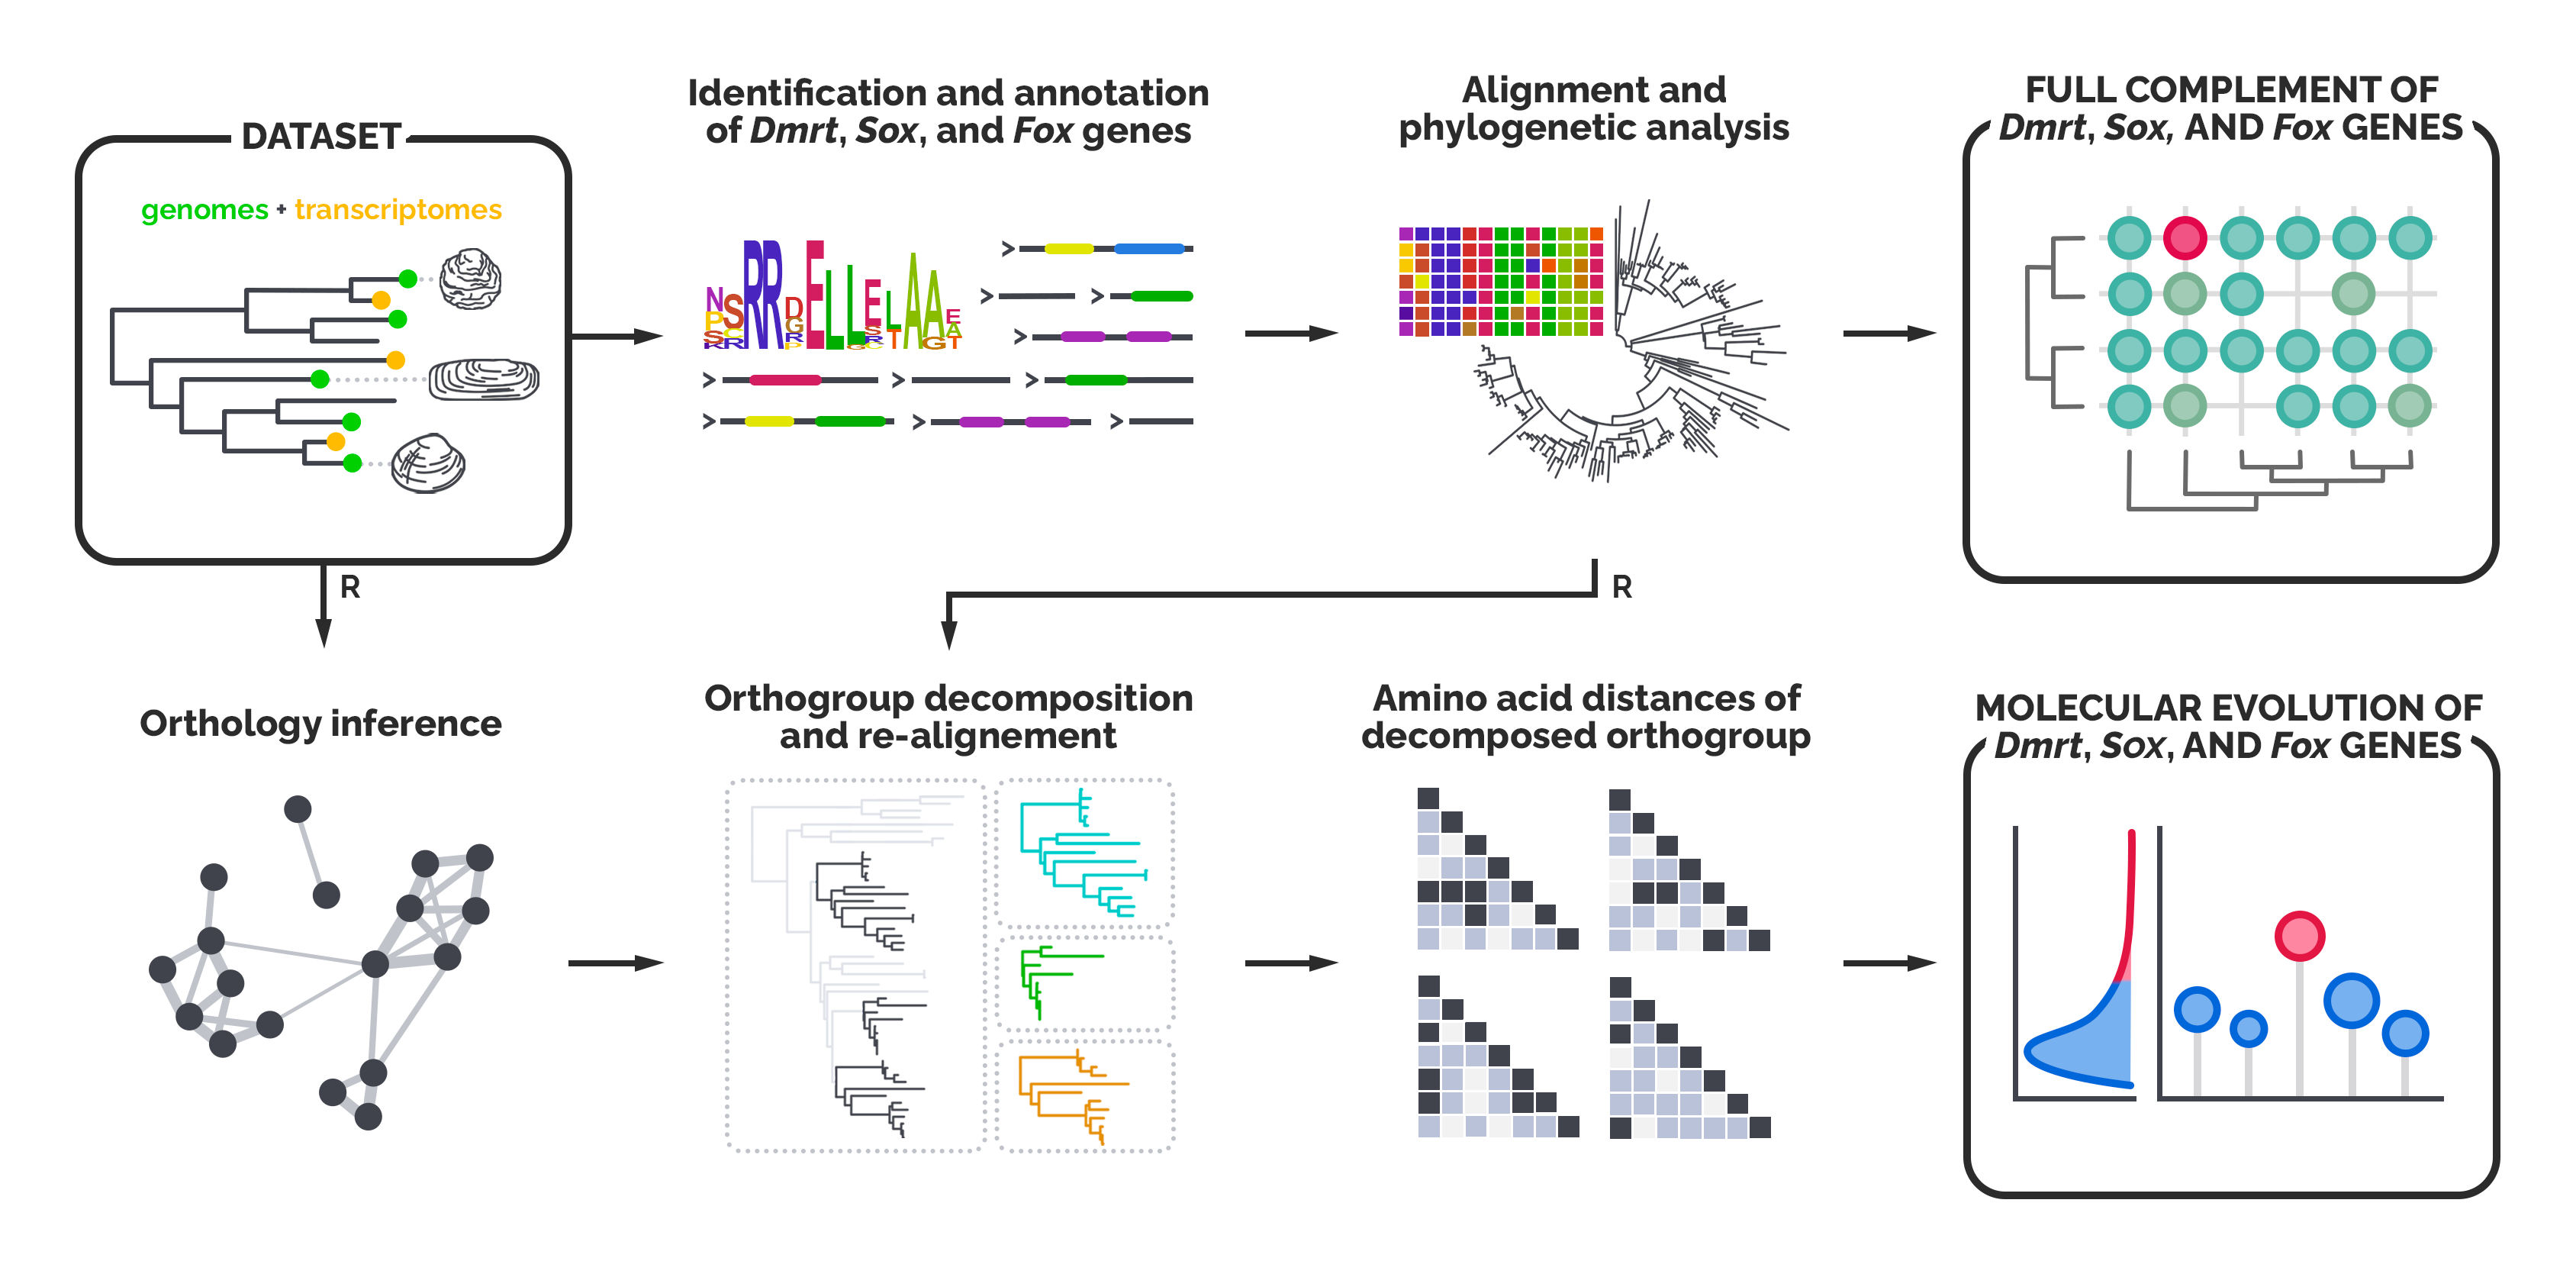
\includegraphics[width=\textwidth]{chapter_inSitu/figure_1.png}
	\caption[\textbf{\gls{pca} of DESeq2-normalised read counts (A) and transcription levels of target and reference genes (B)}]
	{
		\textbf{\gls{pca} of DESeq2-normalised read counts (A) and transcription levels of target and reference genes (B)}. (A) Principal components (PC) 1 and 2 are plotted in the x and y axes, respectively; the proportion of variance explained by each PC is shown in parentheses. Sampled time-points are shown in different colours and are indicated by the hours \glsxtrfull{hpf}. Major developmental transitions are marked with dotted lines. \gls{pca} has been performed on vst-transformed, normalised read counts (DESeq2 median of ratios). (B) Transcription levels of target (\textit{Vasa}, \gls{dmrt-1l}, \textit{Sox-H}, and \textit{Fox-L2}) and reference genes (\textit{Wnt-8a} and \textit{Fox-B2}) as expressed by normalised read counts (DESeq2 median of ratios).
	}
	\label{fig:deseq2}
\end{figure}
\endgroup

Transcription levels of \textit{Vasa}, \glspl{srg}, \textit{Fox-B2}, and \textit{Wnt-8a} were plotted individually (\cref{fig:deseq2-B}) to obtain a proxy of the expected outcome of \gls{hcr}. \textit{Fox-B2} and \textit{Wnt-8a} were employed as control genes to get support for handling of data and of the pipeline, as they were also analysed by \citeboldyearparent{miglioli2024hcrMytilus}. The transcription of both genes starts at \qtylist{4;8}{\hpf}, respectively, reaches a peak at \qty{16}{\hpf}, and then constantly decreases ({fig:deseq2-B}). \textit{Vasa} transcripts are highly abundant in unfertilized oocytes and in embryos \qty{4}{\hpf}, then constantly decrease throughout time; conversely, \textit{Fox-L2} transcripts increase from \qty{12}{\hpf} onward ({fig:deseq2-B}). Both \gls{dmrt-1l} and \textit{Sox-H}, instead, show low or null levels of transcriptions throughout the entire time series ({fig:deseq2-B}).

The maSigPro \gls{dge} analysis of the \gls{mgal} developmental time series found \num{13067} differentially expressed genes (about \qty{17}{\percent} of the analysed genes) and clustered them into 9 different groups, according to their specific transcriptional profiles (\cref{fig:masigpro}). Among the genes of interest, only \textit{Vasa} and \textit{Fox-L2} showed a significantly different transcriptional profile throughout the time series, and were included in clusters 3 and 1, respectively. As already discussed, \textit{Vasa} and \textit{Fox-L2} transcription levels show an opposite tendency, with the former decreasing and the latter increasing throughout time. Both \gls{dmrt-1l} and \textit{Sox-H} were not found to be differentially transcribed by maSigPro and, thus, were not included in any cluster. The same holds true for \textit{Wnt-8a} and \textit{Fox-B2}.

\begin{figure}[t!]
	\centering
	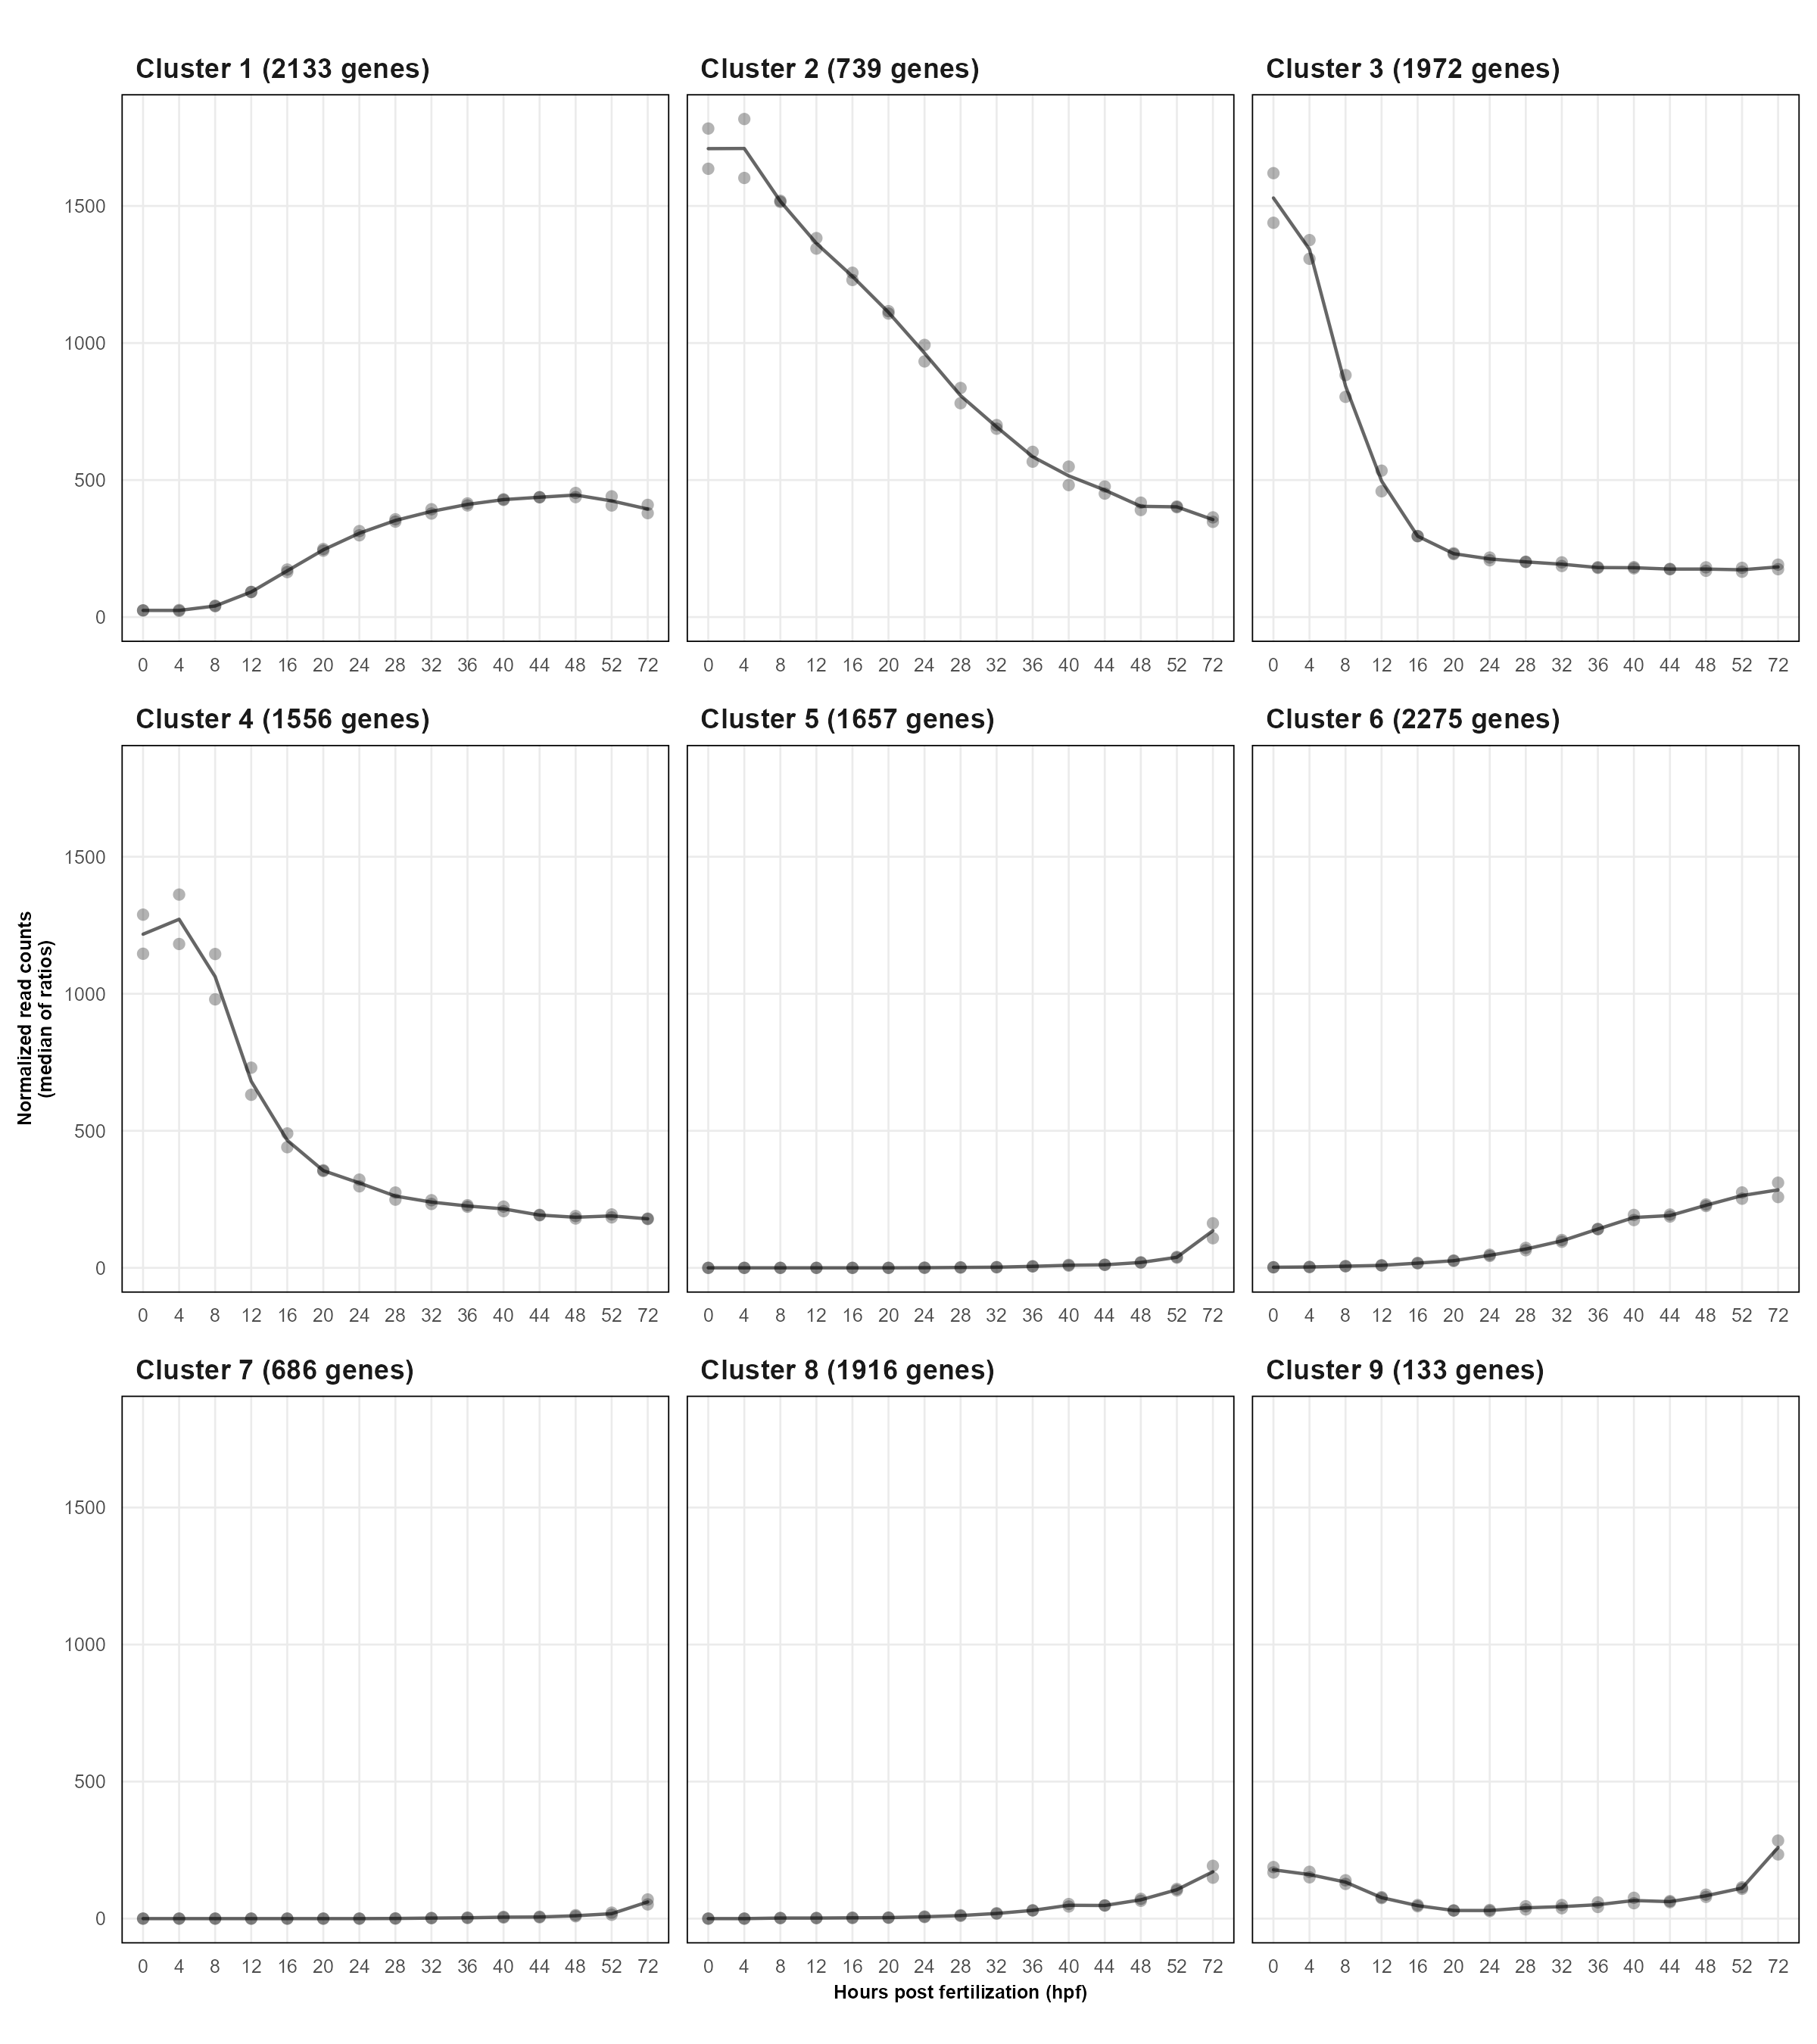
\includegraphics[width=\textwidth]{chapter_inSitu/figure_2.png}
	\caption[\textbf{Transcription patterns of differentially-expressed genes as inferred by maSigPro}]
	{
		\textbf{Transcription patterns of differentially-expressed genes as inferred by maSigPro}. Genes are divided into 9 different clusters according to their transcription patterns throughout 15 sampled time points. Median values of the two biological replicates are shown for each time point and represented by points. Mean values are shown for each time point and represented by solid lines.
	}
	\label{fig:masigpro}
\end{figure}

\afterpage{
\footnotesize
\begin{longtable}[c]{llrrrr}
    \caption[\textbf{Number of imaged samples, divided by developmental stage, experiment, and sex}]
    {
        \textbf{Number of imaged samples, divided by developmental stage, experiment, and sex}.
    }
    \label{tab:embryo_count}\\
    %
    \toprule
    \textbf{Stage}                & \textbf{Experiment}               & \textbf{Females} & \textbf{Males} & \textbf{Undetermined} & \textbf{Total} \\* \midrule \midrule
    \endfirsthead
    %
    \toprule
    \textbf{Stage}                & \textbf{Experiment}               & \textbf{Females} & \textbf{Males} & \textbf{Undetermined} & \textbf{Total} \\* \midrule \midrule
    \endhead
    %
    \textbf{Oocytes}              & \textbf{HCR} & \NA     & \NA   & \NA          & \textbf{11}    \\* \midrule
    2-cell embryos       & HCR          & 8                & 9              & 1                     & 18             \\
    4-cell embryos                & HCR          & 9                & 3              & 0                     & 12             \\
    8-cell embryos                & HCR          & 11               & 3              & 0                     & 14             \\
    12-hpf embryos                & HCR          & 7                & 6              & 0                     & 13             \\
    \textbf{Total embryos}        & \textbf{HCR} & \textbf{35}      & \textbf{21}    & \textbf{1}            & \textbf{57}    \\* \midrule
    24-hpf larvae                 & HCR          & 0                & 1              & 11                    & 12             \\
    48-hpf larvae                 & HCR          & 0                & 0              & 11                    & 11             \\
    72-hpf larvae                 & HCR          & 1                & 1              & 8                     & 10             \\
    \textbf{Total larvae}         & \textbf{HCR} & \textbf{1}       & \textbf{2}     & \textbf{30}           & \textbf{33}    \\* \midrule
    \textbf{Oocytes}              & \textbf{Negative control}         & \NA     & \NA   & \NA          & \textbf{5}     \\* \midrule
    2-cell embryos                & Negative control                  & 7                & 2              & 0                     & 9              \\
    4-cell embryos                & Negative control                  & 7                & 2              & 0                     & 9              \\
    8-cell embryos                & Negative control                  & 5                & 1              & 0                     & 6              \\
    12-hpf embryos                & Negative control                  & 0                & 0              & 3                     & 3              \\
    \textbf{Total embryos}        & \textbf{Negative control}         & \textbf{19}      & \textbf{5}     & \textbf{3}            & \textbf{27}    \\* \midrule
    \textbf{Total larvae}         & \textbf{Negative control}         & \textbf{0}       & \textbf{0}     & \textbf{4}            & \textbf{4}     \\* \midrule \midrule
    \textbf{\begin{tabular}[c]{@{}l@{}}Total imaged\\ samples\end{tabular}} & \textbf{All}                      & \textbf{55}      & \textbf{28}    & \textbf{38}           & \textbf{137}  \\* \bottomrule \bottomrule
\end{longtable}
}

\subsection{mRNA \textit{in-situ} HCR of \textit{Vasa} and SRGs}
Overall, a total of 80 adult \gls{mgal} individuals were sampled and staged for thermal-shock induced spawning. Of these, 8 males and 8 females were eventually selected as parents for single (2 of each sex) and multiple (6 of each sex) crosses, on the basis of their gamete quality (i.e., presence sperm motility, and oocyte transparency and rounded shape). MitoTracker labelling was successfully retained in developing embryos of \gls{mgal} until \qty{12}{\hpf}. After that stage, the stained sperm mitochondria were difficult to detect, and so was the dispersal pattern to establish the sexual identity.

After embryo rearing, fixation, and mRNA \textit{in-situ} \gls{hcr} of target genes, a total of 16 oocytes, 81 embryos and 33 mussel larvae were imaged (\cref{tab:embryo_count}). Of these, on the basis of sperm mitochondria dispersal patterns, 55 were females (dispersed pattern), 28 were males (aggregated pattern) and 38 were of indeterminable sex (ambiguous pattern or unlabelled sperm mitochondria). For each stage, negative controls were also imaged (final count of 36), by staining just sperm mitochondria with MitoTracker and nuclei with DAPI, and going through the \gls{hcr} protocol without adding probes in the hybridization step. A total of 137 samples were imaged.

The \singlecurlyquotes{insitu\_probe\_generator} script (\citebold{kuehn2022probegenerator}) generated: (i) 33 probe pairs conjugated with hairpin B1 and ALEXA-488 for \textit{Vasa}; (ii) 32 probe pairs conjugated with hairpin B2 and ALEXA-647 for \gls{dmrt-1l}; (iii) 27 probe pairs conjugated with hairpin B3 and ALEXA-546 for \textit{Sox-H}; and (iv) 28 probe pairs conjugated with hairpin B4 and ALEXA-700 for \textit{Fox-L2} (\cref{tab:fluorescent_dyes,suppTab:HCRprobes}).

\gls{hcr} labelling of genes of interest proved to be concordant with results obtained from RNA-seq analysis (see \cref{chapter:insitu-DGE}). Concerning \textit{Vasa}, it has been detected throughout every sampled stage (\cref{fig:hcr}\textbf{A}): transcripts were identified quite homogeneously in the cytoplasm of unfertilized oocytes, 2-, 4-, and 8-cell embryos; in gastrulae, \textit{Vasa} is located mainly in the ingressed cells; in trochophores, it forms a cup-like structure in the region opposite to the shell-field; in D-larvae, it is mainly retained in two central areas adjacent to the valves (right and left sides of the larvae) in a sort of a comma-shaped region. Concerning \gls{dmrt-1l} (cref{fig:hcr}\textbf{B}), final images were quite noisy and showed putative non-specific staining at the level of embryo external surface and larvae shell, which may have interfered with the true signal of \gls{hcr} for this gene; in any case, no clear labelling distribution pattern was found in embryos of both sexes. \textit{Sox-H} mRNAs (\cref{fig:hcr}\textbf{C}) were not detected during the imaged developmental stages. Conversely, \textit{Fox-L2} transcripts have been detected starting from the 8-cell stage—where they are homogeneously present, to the D-veliger larvae—where they appear to be mostly co-localized with Vasa (\cref{fig:hcr}\textbf{D} and \textbf{E}). Imaging of control samples (i.e., without mRNA \textit{in-situ} staining) can be found in \cref{suppFig:hcrBianco}.

\begin{figure}
    \centering
    \includegraphics[width=\textwidth]{chapter_inSitu/figure_3.png}
    \caption{\textit{Caption on next page.}}
    \label{fig:hcr}
\end{figure}

\begingroup
\captionsetup[figure]{format=hruleformat}
\begin{figure}\ContinuedFloat
    \caption[]
	{
		\textbf{mRNA \textit{in-situ} \gls{hcr} of \textit{Vasa} (A), \gls{dmrt-1l} (B), \textit{Sox-H} (C), \textit{Fox-L2} (D), and \textit{Vasa}+\textit{Fox-L2} (merged; E) in several developmental stages of \gls{mgal}}. Nuclei are shown in white; in the 2-, 4-, and 8-cell stages, nuclei are also marked with numbers; in the 8-cell stage, nuclei of blastomeres in the background are highlighted with dashed circles. Sperm mitochondria, when stained (shown in green), are marked with arrowheads. For 2-cell, 4-cell, 8-cell, and gastrula stages, embryos of both sexes are reported (top rows: females; bottom rows: males). a: anus; h: hinge; nu: oocyte nucleus; pb: polar body; sf: shell field; st: stomodeum. Scale bar: \qty{20}{\um}. \textit{(Figure on previous page.)}
	}
\end{figure}
\endgroup

\subsection{Immunolocalization of Vasa}
To determine whether the commercial polyclonal antibody (ab209710 by Abcam Limited) could successfully bind \gls{mgal} Vasa, we conducted a phylogenetic analysis (\cref{fig:vasaTree-A}) and a multiple sequence alignment inspection (\cref{fig:vasaTree-B}) of Vasa/Ddx4 proteins, along with its paralog Ddx3, starting from the bivalve curated genome and transcriptome dataset analysed in \cref{chapter:molecularEvolution}. We retrieved three different Vasa sequences in the \gls{mgal} genome (\cref{suppTab:vasa_dataset}). Two of them (VDI03911.1 and VDI03912.1) are splicing variants of the same mRNA (acc. no. 10B017427) investigated through \gls{dge} and mRNA \textit{in-situ} \gls{hcr} in previous sections. Both variants are constituted by 17 exons and differ from each other for only eight leading amino acids at the protein N-terminus (\cref{fig:vasaTree-C}). Their \gls{dead/deah-box} and C-terminal domains show high levels of sequence conservation with respect to \gls{drer} Vasa (\cref{fig:vasaTree-C}). Concerning the other Vasa \gls{mgal} sequence (VDI58335.1), it originates from a separate genomic locus and appears very short (105 amino acid positions) if compared to other Vasa from bivalves (\num{> 800}; data not shown). Additionally, it does not exhibit any complete \gls{dead/deah-box} domain (as per CDD domain annotation). This considered, the additional Vasa gene (and its relative protein) may be an artefact due to genome mis-assembly and/or mis-annotation, or a non-functional gene. Thus, we argue that the correct immunolocalization of the \gls{mgal} Vasa proteins should not be affected, and will not be further discussed.

\begin{figure}
	\centering
	\captionsetup[subfigure]{labelformat=nocaption}
	\begin{subfigure}{0\linewidth}
	\caption{}\label{fig:vasaTree-A}
	\end{subfigure}% <----- get rid of space, for proper centering
	\begin{subfigure}{0\linewidth}
    \caption{}\label{fig:vasaTree-B}
    \end{subfigure}% <----- get rid of space, for proper centering
    \begin{subfigure}{0\linewidth}
    \caption{}\label{fig:vasaTree-C}
    \end{subfigure}% <----- get rid of space, for proper centering
    \includegraphics[width=\textwidth]{chapter_inSitu/figure_4.png}
	\caption[\textbf{\gls{pca} of DESeq2-normalised read counts (A) and transcription levels of target and reference genes (B)}]
	{
		\textbf{\gls{ml} phylogenetic tree of Vasa/Ddx3 and Ddx4 proteins from bivalves and reference species (A), along with the amino acid alignment of the relative \gls{dead/deah-box} (B) and of Vasa proteins from \gls{mgal} and reference species (C)}. (A) The tree has been rooted considering the Ddx4 clade as the outgroup. Reference genes from \gls{drer}, \gls{hsap}, \gls{mmus}, \gls{dmel}, and \gls{cele} are marked with an asterisk at the beginning of the tip. Bootstrap values are shown for each node. (B) The alignment of the \gls{dead/deah-box} is shown for each tip. The signature DEAD (Asp-Glu-Ala-Asp) motif can be found at positions 198--201. Vasa sequences from \gls{mgal} are highlighted with a solid rectangle and two asterisks on the right. (C) The alignment of complete Vasa sequences from \gls{mgal}, \gls{drer}, \gls{hsap}, and \gls{dmel} is shown. \gls{cele} has not been included because the species has multiple Vasa orthologs. The signature \gls{dead/deah-box} and C-terminal-associated domains are highlighted with solid rectangles. Note that position coordinates are not the same between (B) and (C). Colours of amino acid residues in both (B) and (C) correspond to the \singlecurlyquotes{Chemistry\_AA} scheme from the R package \singlecurlyquotes{ggmsa}, which highlights the amino acid side-chain chemistry (\citebold{zhou2022ggmsa}). Bivalve species IDs as in \cref{suppTab:bivalve_dataset}. Cele: \glsxtrlong{cele}; Drer: \glsxtrlong{drer}; Dmel: \glsxtrlong{dmel}; Hsap: \glsxtrlong{hsap}; Mmus: \glsxtrlong{mmus}. Full descriptions of gene names, accession numbers, and species can be found in \cref{suppTab:vasa_dataset}.

	}
	\label{fig:vasaTree}
\end{figure}

Unfortunately, the amount of available samples and antibodies for the experiment was limited. Therefore, we managed to acquire just two oocytes, two 2-cell embryos, and one gastrula. Nonetheless, from the obtained images, we found that Vasa proteins are apparently missing from the oocytes, but can be detected at increasing levels on embryos after \qty{4}{\hpf} (\cref{fig:immuno}) and during gastrulation, with a localization matching that of Vasa mRNAs (\cref{fig:vasaTree-A}). Imaging of control samples (i.e., without primary antibody reaction) can be found in \cref{suppFig:immunoBianco}.

\begin{figure}
	\floatbox[{\capbeside\thisfloatsetup{capbesideposition={right,top},capbesidewidth=0.4\textwidth}}]{figure}[\FBwidth]
	{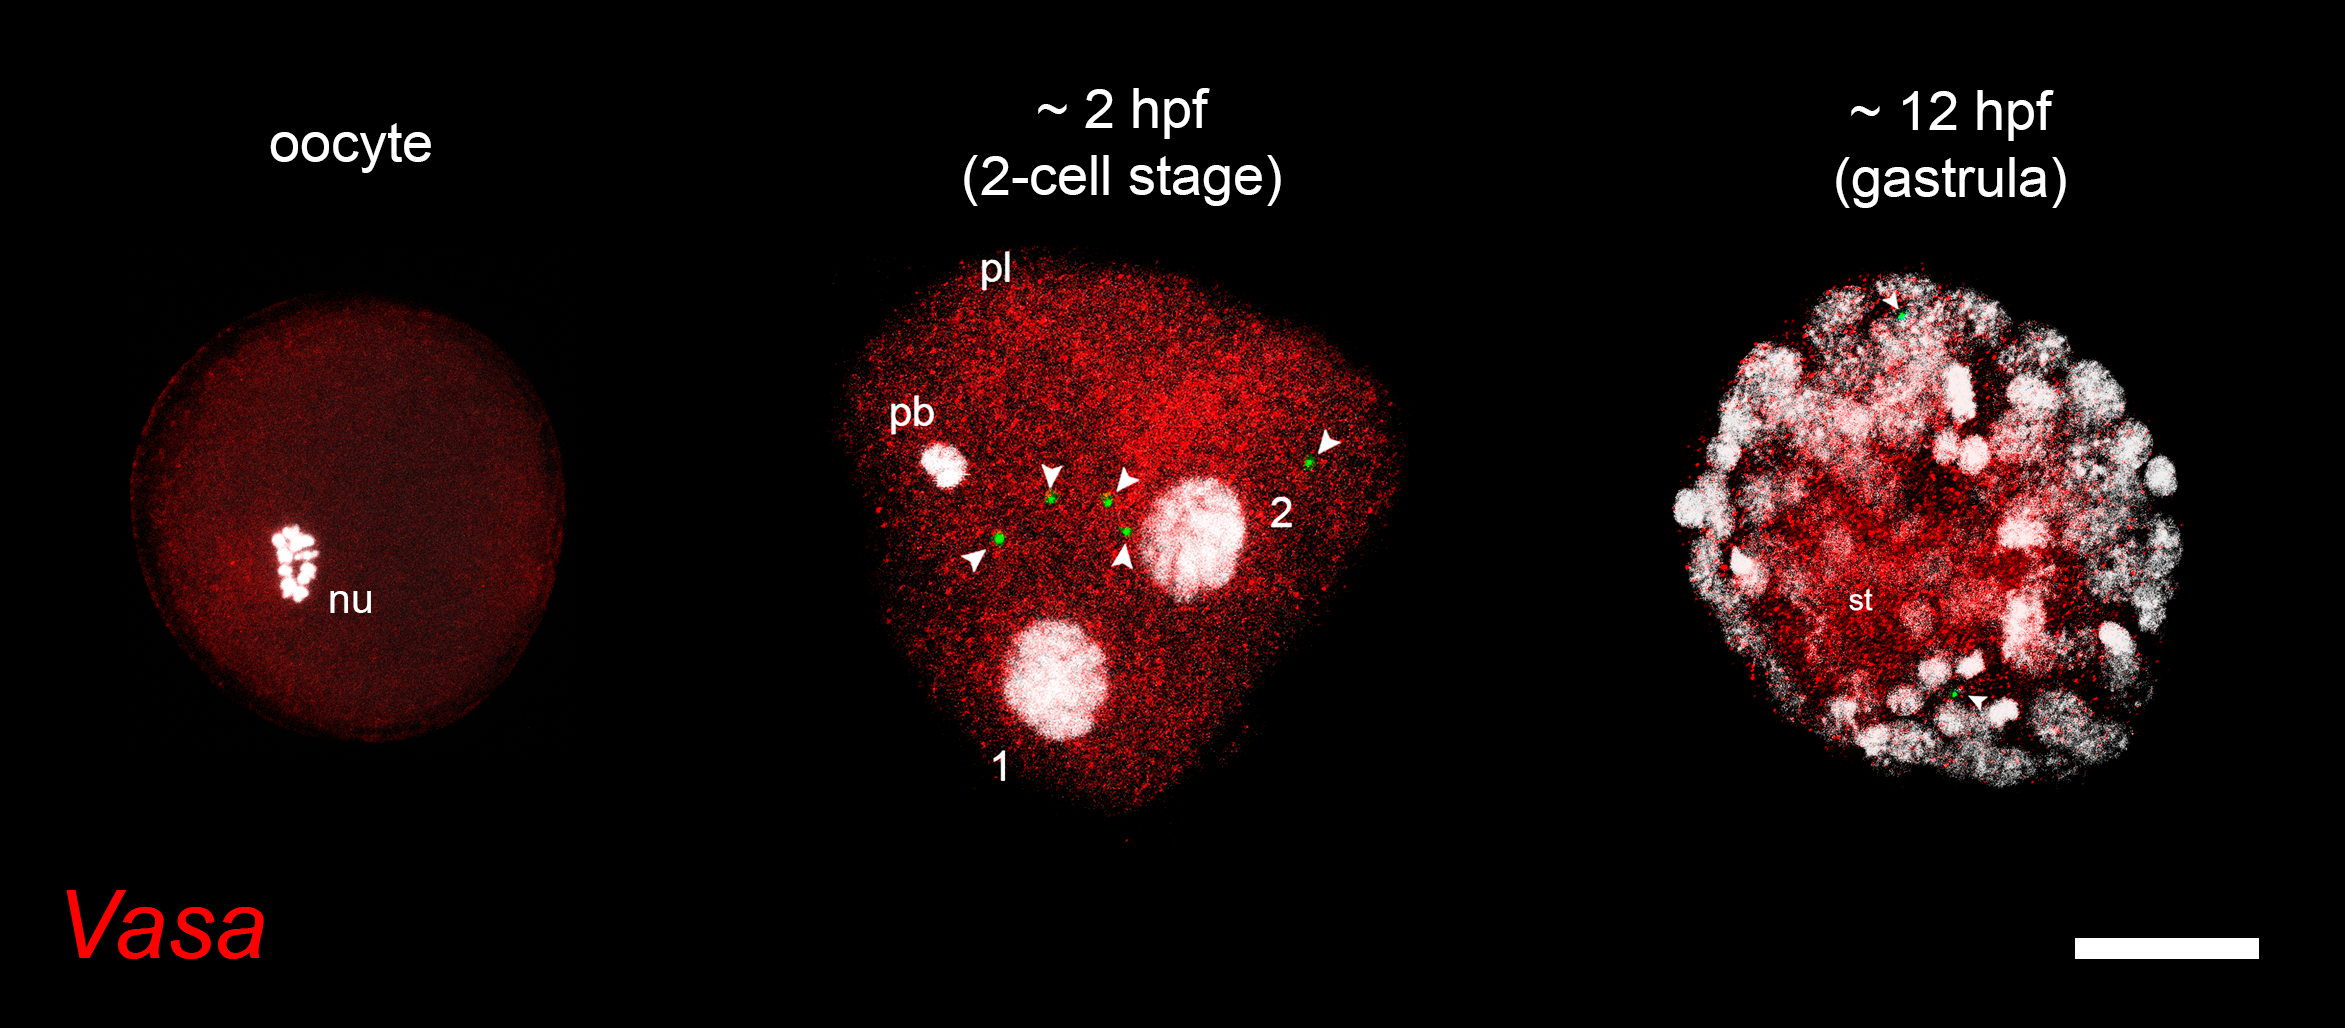
\includegraphics[width=0.55\textwidth]{chapter_inSitu/figure_5.png}}
	{\caption[\textbf{Immunolocalization of Vasa in \gls{mgal} oocyte and embryos}]
	{
		\textbf{Immunolocalization of Vasa in \gls{mgal} oocyte and embryos}. Nuclei are shown in white. Sperm mitochondria (in green) are marked with arrowheads. nu: oocyte nucleus; pl: polar lobe; pb: polar body; st: stomodeum. Scale bar: \qty{20}{\um}.
	}
	\label{fig:immuno}}
\end{figure}

\section{Discussion} \label{chapter:insitu-discussion}
\subsection{Sperm mitochondria are not detected after 12 hpf because of MitoTracker misincorporation or fading}\label{chapter:insitu-discussionMito}
Because of the presence of the unique \gls{dui} of mitochondria, \gls{mgal} offers a compelling system to investigate \gls{sd} during the early stages of embryogenesis. As a matter of fact, the sexual fate of an embryo appears to be established as soon as the first cleavage division, according to the dispersal pattern of sperm mitochondria (\citebold{saavedra1997mytilus,cao2004differential}), despite the two processes are not necessarily causally linked (\citebold{kenchington2009dui}): (i) if the embryo is going to develop into a female, sperm mitochondria can be found scattered across different blastomeres; (ii) if the embryo is going to develop into a male, sperm mitochondria are found aggregated all in the same blastomere (usually the macromere), being subsequently transferred to \glspl{pgc} as part of the germ plasm. Therefore, in order to be able to establish the sexual identity of embryos and link it to any differential transcriptions of \glspl{dsfg}, we labelled sperm mitochondria with MitoTracker (prior to oocyte fertilisation), and check for their dispersal patterns throughout the various sampled stages. Despite being successfully retained in developing embryos up until \qty{12}{\hpf}, the MitoTracker fluorescence was difficult to detect in later stages, and so was the mitochondrial dispersal pattern. This phenomenon may have been caused by: (i) misincorporation of MitoTracker during pre-fertilization sperm incubation (ii) MitoTracker fading after intense manipulation of samples; (iii) MitoTracker dye being incompatible with proper embryo development, i.e., labelled embryos not surviving after \qty{12}{\hpf}.
Based on previous studies showing that MitoTracker labelling of sperm mitochondria (including the relative dispersed and aggregated patterns) can be observed up until the late D-larva stage in \gls{medu} (\qty{72}{\hpf}; \citebold{cao2004differential}), we argue that (i) and (ii) are the most likely explanation for the dye not being detected in samples after \qty{12}{\hpf}, i.e., MitoTracker has not interfered with the correct development of embryos. However, it must be considered that we employed a rosamine-based MitoTracker dye (MitoTracker Red; which better resists aldehydic fixation), while \citeboldyearparent{cao2004differential} used a carbocyanine-based MitoTracker dye (MitoTracker Green). This may have determined different effects on cell vitality, thus making results not comparable to each other. As a matter of fact, despite MitoTracker dyes are life-compatible as per manufacturer\curlyapostrophe s indications, \citeboldyearparent{minamikawa1999chloromethyl} showed that rosamine-based MitoTracker dyes have photosensitising effects on cells. This means that cells labelled with MitoTracker Red may be committed to apoptosis if exposed to intense light, which induce the loss of the mitochondrial membrane potential and consequent mitochondria swelling. However, based on our experimental conditions, we argue that MitoTracker Red photosensitisation has had a minimal effect, if any, on embryo development. As a matter of fact, (i) after sperm MitoTracker staining, samples were kept in the dark throughout the entire sampling period (MitoTracker Red cytotoxicity is not evident in the dark; \citebold{minamikawa1999chloromethyl}), with limited exposure to environmental light just in correspondence with water changes; furthermore, (ii) the photosensitisation has been shown to significantly increase with light doses exceeding \qty{0.4}{\J\per\square\cm} (cell-colony mortality rate of \qtyrange{60}{80}{\percent} compared to control colonies; \citebold{minamikawa1999chloromethyl}), which is higher than typical environmental light exposure (the solar constant is measured at around \qty{1.362}{\kW\per\square\m}, equivalent to \qty{0.1367}{\J\per\square\cm\per\s}); (iii) only a little proportion of mitochondria (the 5 sperm-derived mitochondria) have been labelled with MitoTracker, while the oocyte-derived ones remained unlabelled. Altogether, we think that MitoTracker Red staining did not determine a cytotoxic effect on \gls{mgal} embryos and the consequent survival of only unlabelled embryos. Thus, we conclude that MitoTracker was not properly detected on samples older than \qty{12}{\hpf} because of misincorporation since the beginning or the dye fading. However, we acknowledge that a formal survival and vitality test should be performed on \gls{mgal} embryos marked with MitoTracker Red, in order to exclude any possible cytotoxic effect.

\subsection{Exploring the processes of SD in the \textit{M. galloprovincialis} early development}
To date, the molecular basis of bivalve \gls{sd} has been investigated mainly in adult tissues (e.g., \citebold{li2018foxl2,liang2019sox2,wang2020identification,sun2022examination,wang2022transcriptome}). As a matter of fact, considering that in many bivalve species gonads form anew at the beginning of every reproductive season from several populations of \glspl{pgc} (\citebold{filanti2021early}), it can be speculated that the sexual identity may be established in correspondence with each new gonad formation. This observation would also explain the process by which many bivalve species are capable of sex changes and sex reversal from one reproductive season to the other (\citebold{breton2018sex}). Nonetheless, animal \gls{sd} is a key developmental process often triggered soon after fertilisation and occurring throughout the early development, as can be observed for example in mammals and fruit flies (\citebold{salz2010sex,beukeboom2014evolution,richardson2023comparativeSex}). Consequently, a full understanding of \gls{sd} in bivalves needs to account also for the events taking place during embryo and larval life stages. To our best knowledge, the only investigation of bivalve \glspl{srg} during non-adult stages comes from the Pacific oyster \gls{cgig} (\citebold{naimi2009molecular}), where the transcription levels of \textit{Vasa}, \gls{dmrt-1l}, and \textit{Fox-L2} have been investigated through \gls{qrt-pcr}. In this work, however, only stages between \qty{7}{\dpf} larvae and 4-month-old spats have been tested, and a direct association of the \gls{dmrt-1l}/\textit{Fox-L2} transcription levels with \gls{sd} could not be established. As a matter of fact, sexes cannot be differentiated in oysters before the onset of gametogenesis, and thus the sex of developing embryos/larvae/spats cannot be properly established (\citebold{naimi2009molecular}).

In this work, we aimed to expand the knowledge of bivalve \gls{sd} by investigating for the first time the transcription patterns of three bivalve \gls{sdg} candidates---belonging to the \gls{dsfg} families, during the embryogenesis and early larval development of the Mediterranean mussel \gls{mgal}. This species allows to infer sex of developing embryos by tracing the sperm mitochondria distribution patterns (see \cref{chapter:insitu-introduction,chapter:insitu-discussionMito}). To this purpose, we employed an explorative investigation through a \gls{dge} analysis, and mRNA \textit{in-situ} \gls{hcr}. Our experimental setting, which included the sperm mitochondria labelling, allowed us to \textit{a-priori} establish the sex of developing embryos and larvae, and thus to link any differential transcription pattern of \glspl{dsfg} to the sexual identity.

The \gls{dge} analysis showed that the inferred transcription levels of control genes, \textit{Fox-B2} and \textit{Wnt-8a} (\cref{fig:deseq2-B}), are coherent with the ones reported by \citeboldyearparent{miglioli2024hcrMytilus}, indicating that the results obtained from other genes can be considered reliable. The low or null transcription levels of both \gls{dmrt-1l} and \textit{Sox-H} (\cref{fig:deseq2-B}) may derive from the absence of transcription itself. However, it must be taken into account that \gls{mgal} shows a mather-dependent sex ratio (\citebold{saavedra1997mytilus}), that is, the percentage of females and males in the progeny is tightly linked to the mother\curlyapostrophe s nuclear genome, while being independent from the father\curlyapostrophe s. Thus, considering that \citeboldyearparent{miglioli2024hcrMytilus} do not specify the sex-ratio of the sequenced embryo pool, the possibility that the low expression levels of \gls{dmrt-1l} and \textit{Sox-H} may be caused by some sex-biased related effect cannot be ruled out. Nonetheless, mRNA \textit{in-situ} \gls{hcr} supports also for our samples the scenario depicted by the \gls{dge} analysis, that is, the two genes are likely not transcribed, as no unambiguous signal was detected (\cref{fig:hcr}\textbf{B--C}). Concerning \gls{dmrt-1l}, we think that an additional and more thorough investigation is needed, as the confocal imaging step seemed to have been affected by autofluorescent signals coming from the embryo surface and the larval shell, and/or by a-specific binding  of probes (\cref{fig:hcr}\textbf{B}). Thus, to obtain more reliable results, a new mRNA \textit{in-situ} \gls{hcr} experiment on \gls{dmrt-1l} should be designed, possibly using a set of amplifiers and fluorophores which is different from the ones employed here (B2-647; \cref{tab:fluorescent_dyes}).

The transcription levels of \textit{Fox-L2} are opposed to those of \textit{Vasa} (see \cref{chapter:insitu-results,chapter:insitu-discussionVasa,fig:deseq2-A}): the gene is not transcribed up until about \qty{12}{\hpf}, i.e., corresponding to gastrulation; from this stage onward, the gene transcription is detected homogeneously all over the embryo, and then becomes restricted to two regions located at both sides of the D-veliger larvae (\cref{fig:hcr}\textbf{D}). In particular, in this stage of development, \textit{Fox-L2} appears to be co-localised with Vasa (\cref{fig:hcr}\textbf{E}), suggesting a role in \gls{pgc} specification and/or differentiation. No sex-biased transcription has been detected for \textit{Fox-L2}, though it must be considered that after \qty{12}{\hpf} we were not able to confidently establish the sexual identity of embryos/larvae through the localization of sperm-derived mitochondria (see \cref{chapter:insitu-discussionMito}). Thus, although it is tempting to speculate a possible role of \textit{Fox-L2} in the specification of female gonads, as proposed by \citeboldyearparent{zhang2014genomic} in \gls{cgig}, no definitive conclusions can be drawn at this time.

All considered, this work suggests two scenarios: (1) \gls{dmrt-1l}, \textit{Sox-H}, and/or \textit{Fox-L2} are truly \glspl{sdg}, or in any case are top regulators in the bivalve \gls{sd} process (as proposed by previous authors [\citebold{zhang2014genomic,li2018foxl2}] and by the comparative genomics analysis of \cref{chapter:molecularEvolution}), though in \gls{mgal} \gls{sd} (hence, their activation) does not occur in early development, but in later stages; (2) \gls{dmrt-1l}, \textit{Sox-H}, and \textit{Fox-L2} are not \glspl{sdg}, but are involved in gonad differentiation and maintenance in adult individuals. That said, the two possibilities should not be viewed as mutually exclusive. As a matter of fact, \gls{dmrt-1l}, \textit{Sox-H}, and/or \textit{Fox-L2} may be required during \gls{mgal} development for early \gls{sd}, which however occur at advanced larval/spat stages, as observed in \gls{cgig} (\gls{sd} occurs at \qtyrange{40}{60}{\dpf}; \citebold{naimi2009molecular,santerre2013oyster}), but they are also required in adults to allow \glspl{pgc} to initiate the sex-specific gonad development and differentiation at every reproductive season. As a matter of fact, a similar expression pattern has been seen for \gls{mgal} \textit{vasa}, whose transcription is detectable in \glspl{pgc} (i) at a low level during the non-reproductive season, and (ii) at a high level both in immature mussels and in the reproductive season (\citebold{obata2010PCGproliferation}). Thus, it can be speculated that the genes triggering the \gls{sd} cascade may be following similar paths.

\subsection{Primordial germ cells are specified by both preformation and epigenesis in \textit{M. galloprovincialis}}\label{chapter:insitu-discussionVasa}
The process of gonad specification (including \glspl{pgc}) in bivalves have been studied in several species, both in adults (e.g., \citebold{fabioux2004oysterAdult,obata2010PCGproliferation,filanti2021early}) and during early development (\citebold{woods1932sphaerium,fabioux2004oysterEmbryo,kakoi2008vasaSaccostrea}). In the pea clam \gls{sstr} (\citebold{woods1932sphaerium}), the specification of the germline is traced back to the unfertilized oocyte, where the germline determinants (in the form of electron-dense granules, mainly containing mitochondria) are included in an asymmetric region of the cytoplasm (the germ plasm). The zygote segmentation then segregates the germ plasm in single blastomeres, until in the gastrula it is found only in two quiescent \glspl{pgc}, which derives from the 4d blastomere (nomenclature as per \citebold{lyons2012cleavage}). In the Pacific oyster \gls{cgig} (\citebold{fabioux2004oysterEmbryo}), a similar process of \gls{pgc} formation has been described. The germline marker \textit{Vasa} is found to be maternally transmitted to the embryo and deposited in a region (the germ plasm) at the vegetal pole of the oocyte. With the onset of segmentation, \textit{Vasa} progressively segregates in single blastomeres, until it is found only in two separated cell clumps at both sides of the pericardic region in the D-larva (\cref{fig:vasaComparison-A}), where they will form \glspl{pgc}. The two cell clumps derive again from the 4d blastomere and, in adult oysters, they will periodically proliferate and migrate to the adjacent connective tissue to build gonad acini during the reproductive season (\citebold{fabioux2004oysterAdult,milani2017vasa}). A different mechanism has instead been proposed for the Japanese spiny oyster \gls{skeg} (\citebold{kakoi2008vasaSaccostrea}). Here, \textit{Vasa} is said to be transcribed all over the embryo until the 8-cell stage (data are not available on the original publication), becoming progressively more restricted to certain blastomeres only after the 50-cell stage. With gastrulation, \textit{Vasa} is detected only at the posterior mesoderm, which derives from the 4d blastomere. In the present work, in the attempt to investigate the transcription patterns of several \glspl{sdg}, we also characterised the emergence of \glspl{pgc} in the early development of \gls{mgal} by mean of Vasa/Vasa localization, thus providing an additional description of \gls{pgc} development in bivalves.

\begingroup
\captionsetup[figure]{format=hruleformat}
\begin{figure}
    \centering
    \captionsetup[subfigure]{labelformat=nocaption}
	\begin{subfigure}{0\linewidth}
	\caption{}\label{fig:vasaComparison-A}
	\end{subfigure}% <----- get rid of space, for proper centering
	\begin{subfigure}{0\linewidth}
    \caption{}\label{fig:vasaComparison-B}
    \end{subfigure}% <----- get rid of space, for proper centering
	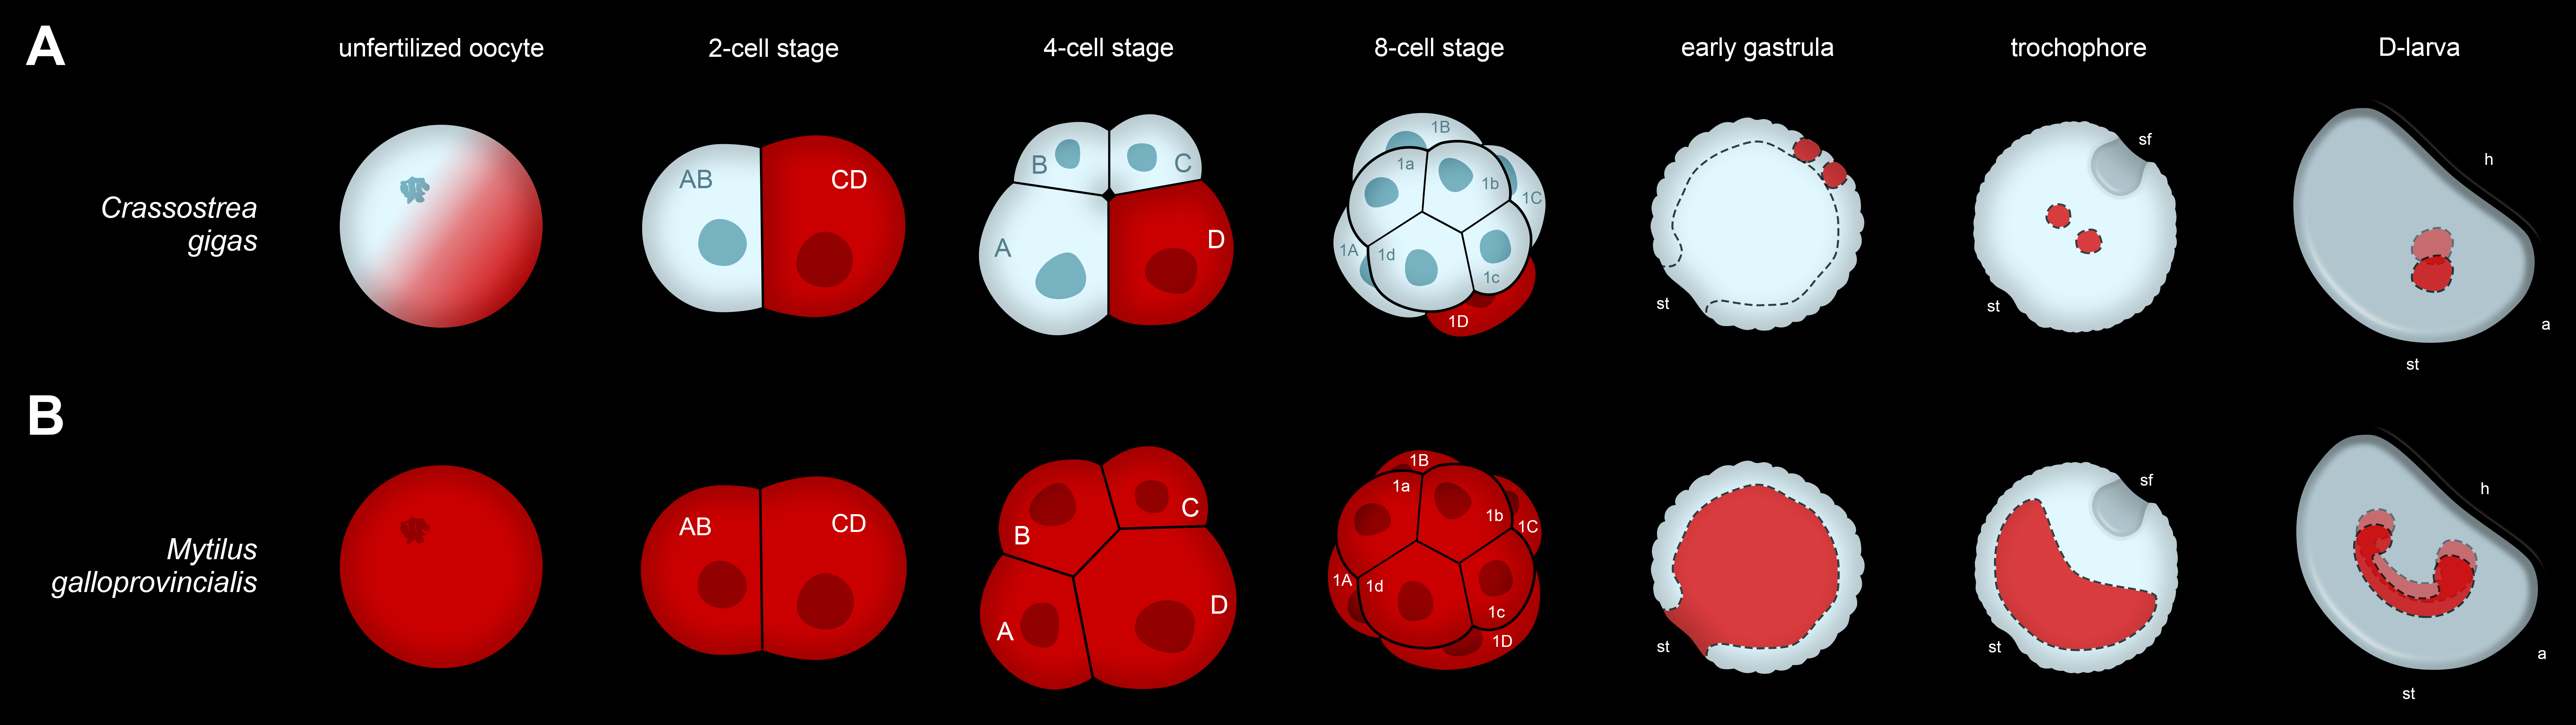
\includegraphics[width=\textwidth]{chapter_inSitu/figure_6.png}
	\caption[\textbf{Comparison of Vasa localization (in red) during the Pacific oyster \gls{cgig} (A) and the Mediterranean mussel \gls{mgal} (B) early development}]
	{
		\textbf{Comparison of Vasa localization (in red) during the Pacific oyster \gls{cgig} (A) and the Mediterranean mussel \gls{mgal} (B) early development}. Drawings not in scale. Data of \gls{cgig} from \citeboldyearparent{fabioux2004oysterEmbryo}. Blastomere nomenclature as per \citeboldyearparent{lyons2012cleavage}. a: anus; h: hinge; st: stomodeum; sf: shell field.
	}
	\label{fig:vasaComparison}
\end{figure}
\endgroup

According to the \gls{dge} analysis, \textit{Vasa} shows a transcription pattern typical of maternal factors (\citebold{xu2018oocyte}), which are stored as transcripts in the oocytes during oogenesis and then constantly decrease throughout embryo segmentation, gastrulation and early larval development, down to undetectable levels (\cref{fig:deseq2-B}). mRNA \textit{in-situ} \gls{hcr} confirmed these results, showing that \textit{Vasa} mRNA is located all over the cytoplasm of the oocyte and in all the blastomeres up until the gastrulation stage, when cells positive to Vasa move to constitute internal cell layers; following additional morphogenetic movements, \textit{Vasa}-positive cells are eventually present only in two limited regions at both the lateral sides of the D-veliger (\cref{fig:hcr}\textbf{A}). On the contrary, immunolocalization showed a different temporal distribution pattern compared to its mRNA, revealing that Vasa does not occur in the oocyte, but that its translation begins only in the late segmentation stages of the zygote and then increases with gastrulation (\cref{fig:immuno}). This different localisation is likely the result of a delay in \textit{Vasa} mRNA translation, which is activated only during the embryo segmentation and grows with the increase of cell number. Nonetheless, this different localisation pattern of mRNA and protein may also have been determined by the differential transcription/translation of the two \textit{Vasa} splicing variants annotated in the \gls{mgal} genome, or by a non-specific binding of either the \gls{hcr} DNA probes or the primary polyclonal antibody. However, considering that the two \textit{Vasa}/Vasa variants are mostly identical, except for eight leading amino acids at the protein N-terminus (\cref{fig:vasaTree-C}), in our experiments we should have been able to target both. As a matter of fact, identifying any differential expression between the two variants would be almost impossible, either through mRNA \textit{in-situ} \gls{hcr} or immunolocalization. Accordingly, the \gls{dge} analyses failed in retrieving any dissimilarity in the transcription levels of the two splicing variants (data not shown), as the experiment was based on short-read sequencing (\citebold{miglioli2024hcrMytilus}). Regarding the \gls{hcr} probes, they have been specifically designed on the complete \textit{Vasa} mRNA spliced sequence, which has already been proven to specifically label \glspl{pgc} in a previous analysis on \gls{mgal} sub-adults and adults individuals (\citebold{obata2010PCGproliferation}). Regarding the commercial antibody, given the high sequence similarity between the Vasa proteins from \gls{mgal} and \gls{drer} (the protein used to produce the antibody; see \cref{chapter:insitu-MM}), at least in their core regions (i.e., the \gls{dead/deah-box} and the C-terminal domains; \cref{fig:vasaTree-C}), we are confident that the immunolocalization procedure correctly labelled Vasa proteins; furthermore, the same set of polyclonal antibodies has been shown to successfully target \glspl{pgc}/\glspl{gc} in another bivalve species, \gls{rphi}, and its specificity has been supported by Western blotting (\cite{filanti2021early}). We thus consider our results to be strongly reliable in the correct localization of \textit{Vasa}/Vasa.

Altogether, the present study shows a process of germline specification in the Mediterranean mussel which resembles that of \gls{skeg}, but differs from the one described in \gls{cgig} (\cref{fig:vasaComparison-A}) and \gls{sstr}. As a matter of fact, contrary to these latter two species, in \gls{mgal} \textit{Vasa} transcripts do not form any evident gradient in the oocyte and early stages of embryogenesis (until 8-cell stage), while becoming progressively more restricted to specific cell populations only later in development (cref{hcr, fig:vasaComparison-B}). Particularly, with the onset of gastrulation, \textit{Vasa}-positive cells are internalised in the developing gastrula, and \textit{Vasa} is thus retained only by the inner cell layers. Once the embryo metamorphoses into a trochophore larva, \textit{Vasa} transcripts arrange in a cup-like structure in the region opposite to the shell field (the ventral side), while in the early D-veliger \textit{Vasa} is present only in two lateral regions next to the valves. Here, \glspl{pgc} are going to form, eventually constituting two symmetrical linear clumps at the base of the dorsal mantle (\citebold{obata2010PCGproliferation}), which is going to represent the primary source of stem cells for gonad acini formation at every reproductive season (\citebold{obata2010PCGproliferation}). This mechanism is also reflected in the localization of Vasa proteins, which do not show any clear gradient in the oocyte---from which is absent, and at least up until gastrulation. Altogether, these findings suggest that in the Mediterranean mussel, \textit{Vasa}/Vasa may segregate in the \glspl{pgc} not only because of their inheritance as maternal factors (through preformation), but also in response to some external (and unknown) zygotic signal (through epigenesis). Therefore, \textit{Vasa} alone do not allow to identify the \glspl{ppgc} or the \glspl{pgc} during the earliest stages of development, as instead it has been shown in adult individuals (i.e., upon \gls{pgc} formation; \citebold{obata2010PCGproliferation}). Given that \textit{Vasa}/Vasa mark a population of cells instead of few blastomeres (those constituting the \glspl{ppgc}), Vasa may consequently play a role also in the broader field of stem cell specification during embryogenesis, as shown in the marine polychaete \gls{pdum} (\citebold{rebscher2007vasa}) and the sea urchin \gls{spur} (\citebold{voronina2008vasa}). In these two species, the germline is specified via an intermediate process relying on both preformation and epigenesis, which can be considered a \singlecurlyquotes{two-step process} (\citebold{rebscher2007vasa,kumano2015evolution}). In this model, a lineage of \glspl{psc} first segregates during early embryogenesis, and then produces \glspl{pgc} and other mesodermal somatic structures by unequal cell division. The germline markers, including \textit{Vasa}, are localised in both the \glspl{psc} and in the descendant \glspl{pgc}. A similar pattern of \textit{Vasa} localisation (i.e., ubiquitously present in oocytes and during early cleavage of the embryo, then progressively restricted to specific blastomeres) has also been shown in the snail \gls{iobs} (\citebold{swartz2008vasaIlyanessa}) and the abalone \gls{hasi} (\citebold{kranz2010vasaHaliotis}), despite not being directly linked to \gls{psc} specification.

\section{Conclusion}\label{chapter:insitu-conclusions}
In the present work, we hypothesise that the \gls{pgc} specification in \gls{mgal} follows a two-step process (i.e., a combination of both preformation and epigenesis), which involves the \glspl{pgc} to be formed only after embryogenesis (\citebold{kumano2015evolution}). A similar process may also be hypothesised for \gls{skeg} (\citebold{kakoi2008vasaSaccostrea}). This mechanism may also explain why \gls{dmrt-1l} and \textit{Sox-H}, if confirmed as \glspl{sdg}, are not transcribed during the investigated developmental stages. \gls{sd} would in fact happen only upon \gls{pgc} commitment, thus during advanced larval development. The present work also represents the first attempt to characterise the spatial localisation of three \glspl{dsfg} in the Mediterranean mussel embryonic and larval develpoment, along with \textit{Vasa}/Vasa, and proves the importance of considering also the developmental stages when investigating new species in a comparative framework. Adopting such an evolutionary developmental perspective may in fact reveal new processes and patterns in animal biology, even when considering related species. As a matter of fact, on the basis of available studies, it has been previously proposed that \gls{pgc} specification is generally based on epigenesis in gastropods and preformation in bivalves (\citebold{obata2012PCGspecification_molluscs}), even though the underlying mechanisms may be species-specific (\citebold{obata2012PCGspecification_molluscs}). However, the model represented by the Mediterranean mussel showed that the process of \gls{pgc} specification may be more diverse in bivalves than expected: preformation happens in \gls{cgig} and \gls{sstr}, and the two-step process happens instead in \gls{skeg}, and, as we propose, in \gls{mgal}. Therefore, results provided by the present work support the idea that the traditional preformation and epigenesis should not be accounted as mutually-exclusive phenomena nor as the only mechanisms of \gls{pgc} formation (\citebold{extavour2007evolutionGermline,kumano2015evolution}). Clearly, given the unavailability of any \gls{pgc} marker in bivalve embryos and larvae (and in mollusc in general), at the moment it is not possible to unambiguously establish the emergence and commitment of \glspl{pgc} during embryogenesis (\citebold{rebscher2014establishing}), especially if based only on few germline genes. As a matter of fact, \glspl{pgc} may share certain genetic markers (e.g., \textit{Vasa}, \textit{Nanos}, \textit{Piwi}, and \textit{Pl-10}) also with some stem cell lineages (\citebold{extavour2003mechanisms,extavour2007evolutionGermline,rebscher2007vasa,voronina2008vasa,rebscher2014establishing,piccinini2023germline}). Thus, more comprehensive investigations are needed to fully and unambiguously characterise the emergence of the germline in bivalve embryos, for example through the examination of the histological and cytological morphology and of genetic regulations (\citebold{extavour2003mechanisms}). A similar scenario holds true also for \gls{sd} and \glspl{sdg}. In fact, we should not expect that the sex-determining process, together with its underlying gene regulatory networks and the timing of its expression, is the same across the entire bivalve diversity. \gls{sd} is indeed one of the most variable developmental processes, despite its importance in the morphological development of an organism (\citebold{capel2017vertebrate}). However, it can be expected that the main actors, being them genetics or environmental or of multiple origin, are conserved, at least in having a role along the whole \gls{sd} process (\citebold{capel2017vertebrate}). Future studies would thus need to further address the functions of the main \gls{dsfg} candidates, as well as the modes of \gls{sd} and germline development, through cutting-edge techniques (such as single-cell RNA-sequencing) and possibly also encompassing various life stages. In this sense, it is tempting to consolidate the role of the Mediterranean mussel as a model system for \gls{sd} and germline studies by taking advantage not only of the \gls{dui} of mitochondria as a proxy for the sexual identity, but also of the ability of the species to produce a sex-biased offspring with the sole maternal influence (\citebold{saavedra1997mytilus}). This would allow a more thorough and straightforward investigation of the determinants influencing the sex and germline specification of developing mussels, by means of targeted RNA-sequencing and transcript/protein localisation.

% \end{document}
